\section{multilet}
Multilet has been implemented like so:\\
First off, implement the lexer as to recognize semicolons like so:\\
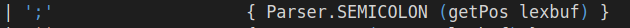
\includegraphics[width=\linewidth]{Materials/Lexer/MultiletLexer}
When the lexer recognizes the semicolon, it parses it to the parser and matches it with the following statement:\\
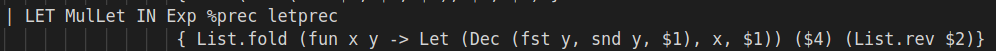
\includegraphics[width=\linewidth]{Materials/Parser/MultiletMatch}
The definition of multlet is given in the following, recursive function:\\
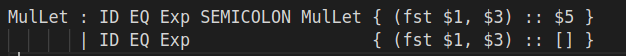
\includegraphics[width=\linewidth]{Materials/Parser/MultiletParser}\\
This function adds the given ID and Expression to a list. If a semicolon is met, the function is called again as there are more let-bindings to add to the list. If no semicolon is met, the ID and expression is added to an empty list as to stop the recursive calls since there are no more let-bindings to be made and the next keyword is expected to be IN. Afterwards, we call our let-function on each element in the list. When finished, we have succesfully bounded multiple IDs with multiple expressions.  
